% Supplement to varneb_CPC.tex; compile from this project directory.
\documentclass[10pt,a4paper]{article}
\usepackage[margin=18mm]{geometry}
\usepackage{graphicx}
\usepackage{amsmath}
\usepackage{caption}
\graphicspath{{figures/}}
\begin{document}
\begin{center}
{\Large Supplementary information for VARNEB}\par
\vspace{4pt}
{\small Xudong Zhu and VARNEB contributors}
\end{center}

\section*{Supplementary Figure S1. Material-path controls}
\begin{figure}[h]
\centering
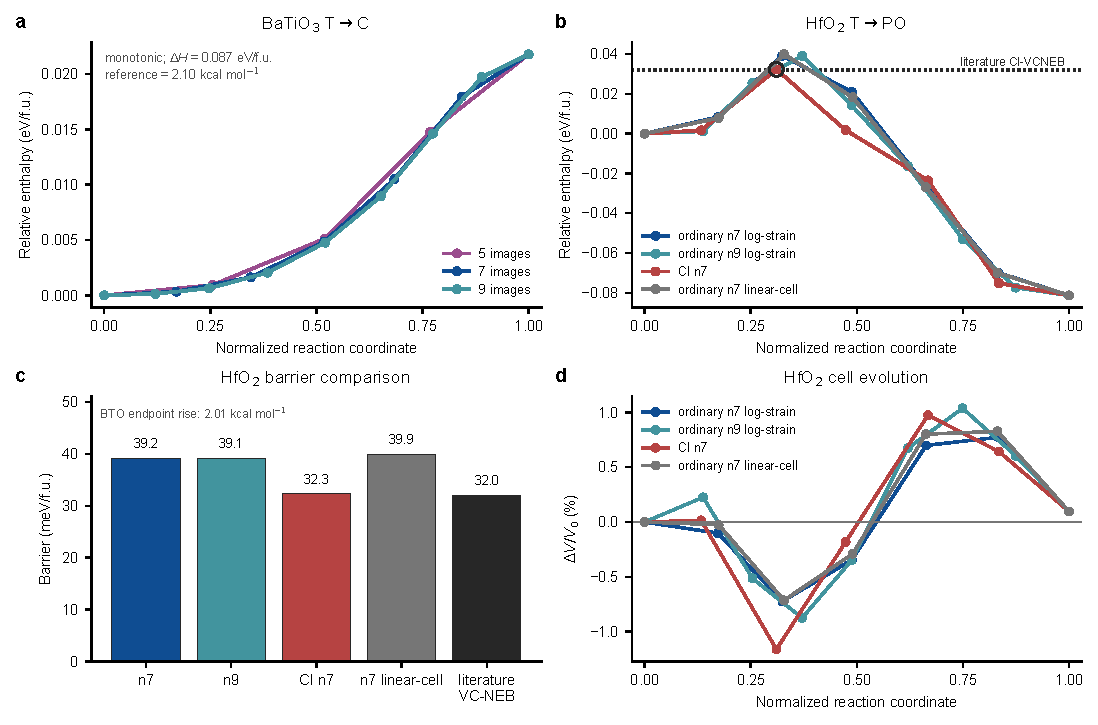
\includegraphics[width=0.98\textwidth]{vcneb_material_validation.pdf}
\caption*{\textbf{S1.} Material paths and qualified literature comparison.
(a) ABACUS/PBE BaTiO$_3$ T-to-C at 5, 7, and 9 total images: the monotonic
0.08713-eV/BTO endpoint rise is not an activation barrier. (b) HfO$_2$
T-to-PO log-strain paths, linear-cell control, and staged climbing-image
refinement; the open circle marks the climbing image and the dotted line an
external literature barrier. (c) HfO$_2$ barriers per formula unit; the
literature bar is not a statistical replicate. (d) Relative volume along the
variable-cell paths. The BTO and HfO$_2$ calculator contracts and the
limitations of cross-functional comparisons are stated in the main text.}
\end{figure}

\clearpage
\section*{Supplementary Figure S2. GaN endpoint-mode and strain evolution}
\begin{figure}[h]
\centering
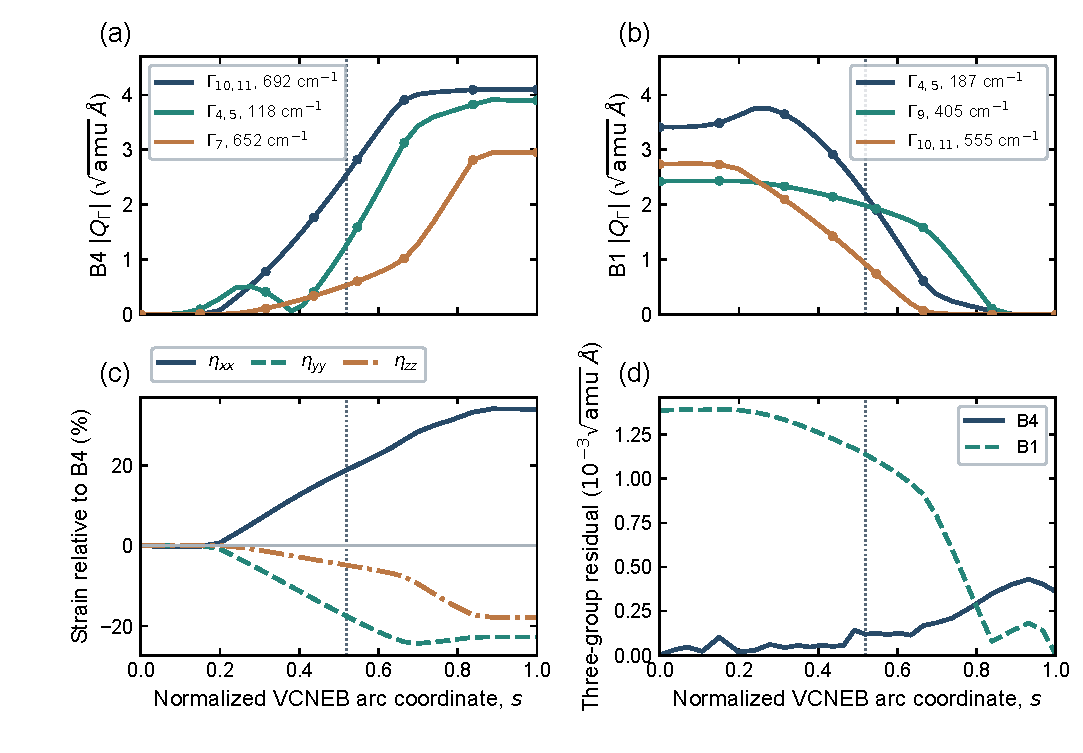
\includegraphics[width=0.96\textwidth]{gan_gamma_path_600eV.pdf}
\caption*{\textbf{S2.} All-image GaN B4-to-B1 mode and strain evolution at
45.7 GPa, using the original VASP/PBE 600-eV electronic contract and
independent $1\times1\times1$ endpoint $\Gamma$ force constants. The 29
total images share one normalized variable-cell path coordinate. (a,b)
Atomic displacement norms in the three leading optical $\Gamma$ subspaces
of B4 and B1, respectively; the labels rank each endpoint basis separately
and do not identify modes across phases. (c) Symmetric strain relative to
B4. (d) Atomic reconstruction residual after those three groups; the
ordinate is in $10^{-3}\sqrt{\mathrm{amu}}\,\text{\AA}$. The dotted line
marks the highest discrete image (15), not a certified stationary saddle.
Mode amplitudes are geometric projections, not barrier contributions. The
29-row source data and input-hash audit accompany the project archive.}
\end{figure}
\clearpage
\section*{Supplementary Figure S3. Local GaN Hessian and endpoint-mode projections}
\begin{figure}[h]
\centering
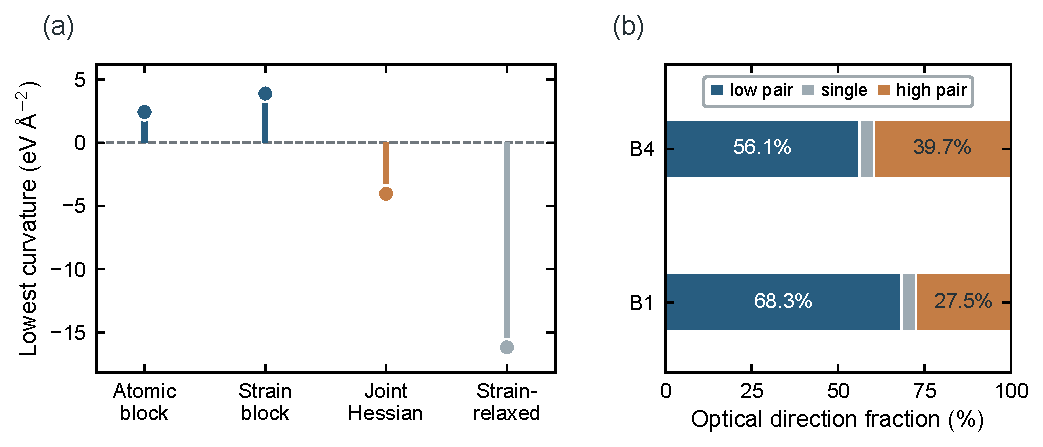
\includegraphics[width=0.96\textwidth]{gan_joint_mode_600eV.pdf}
\caption*{\textbf{S3.} Local atom--strain coupling at 45.7 GPa, under the
original VASP/PBE 600-eV contract. (a) Lowest curvatures of the
frozen-strain atomic and frozen-atomic strain blocks, full joint Hessian,
and strain-relaxed Schur complement at a 0.02-\AA{} step. Translation-free
coordinates use $\mathrm{cell\_scale}=3.3983$ \AA; curvature magnitudes
depend on this metric. (b) Squared geometric projections of the joint
negative direction's atomic optical component onto independent B4 and B1
endpoint $\Gamma$ groups, ranked separately by frequency. These overlaps
are not mode-resolved barrier shares. The energy--force mismatch and
incomplete stationary-point tests preclude certification of a strict
variable-cell transition state.}
\end{figure}
\clearpage
\section*{Supplementary Figure S4. Frozen cubic BTO soft-mode grid}
\begin{figure}[h]
\centering
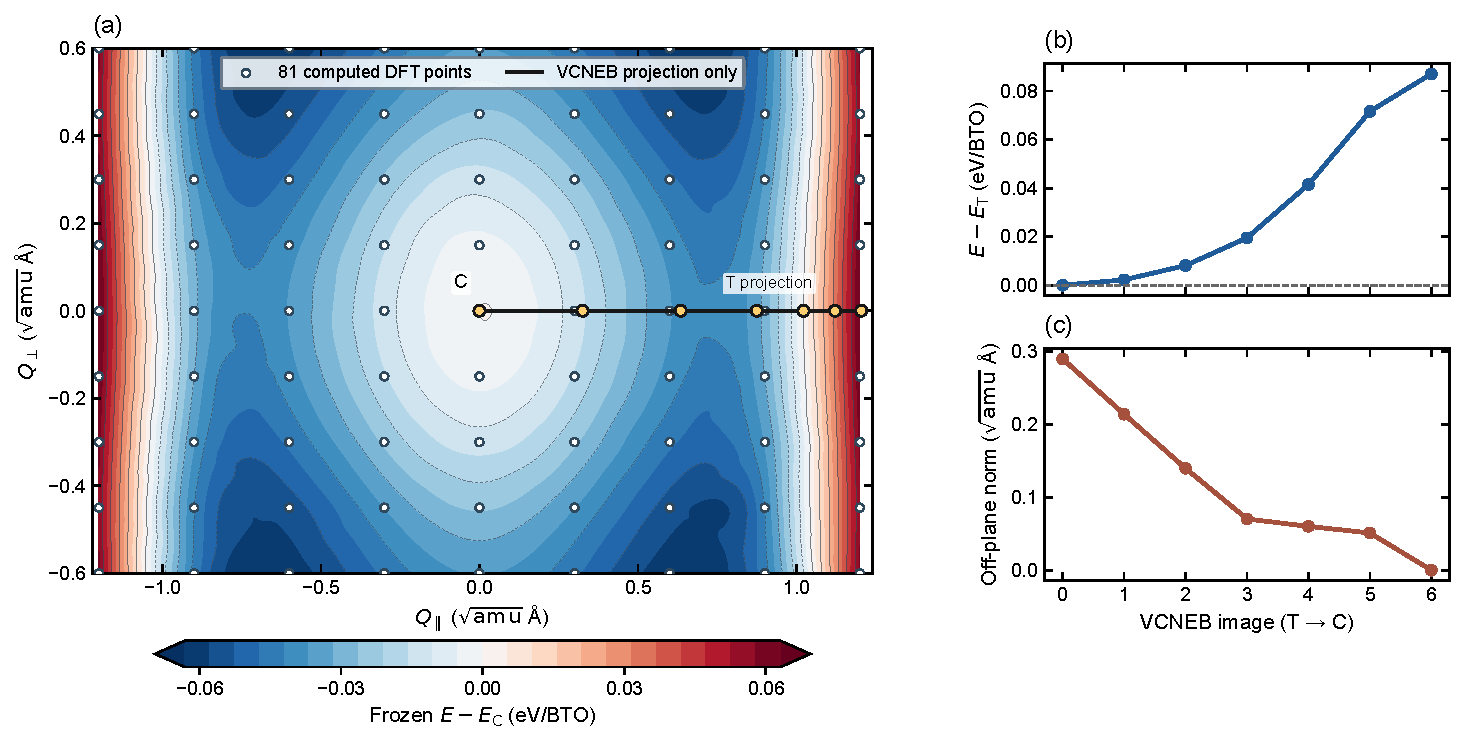
\includegraphics[width=0.98\textwidth]{bto_frozen_soft_mode_81_20260928.pdf}
\caption*{\textbf{S4.} Exploratory cubic-cell BTO two-soft-mode cut, distinct
from the symmetry-restricted variable-cell sheet in main Fig.~2. ABACUS/PBE
static calculations use the unchanged 100-Ry/10-au-DZP basis and
$4\times4\times4$ electronic mesh; the mode axes derive from the cubic
$1\times1\times1$ $\Gamma$ calculation. (a) The 81 circles are measured
DFT energies on a complete $9\times9$ $(Q_\parallel,Q_\perp)$ grid;
the smooth color field is display interpolation, not additional DFT.
The black line is only the seven-image T-to-C VCNEB projection onto this
frozen plane. (b) Actual variable-cell path energies relative to T.
(c) Atomic displacement norm omitted by the plane. The prior 59-point
interpolation predicted the 22 newly computed grid nodes within 0.441
meV/BTO, whereas full-grid interior leave-one-out error reaches 5.14
meV/BTO and the display interpolant undershoots a measured minimum by
1.78 meV/BTO. Neither the interpolated minimum nor a point on the
projected line is a relaxed T-to-C barrier.}
\end{figure}
\end{document}
